In diesem Kapitel wird zunächst die Hochfrequenzmethode zur Bestimmung der Energiedifferenz erklärt und dann das konkrete Vorgehen bei der Versuchsdurchführung.

\subsection{Hochfrequenzmethode}
Nachdem sich die Besetzungsinversion eingestellt hat, gibt es zwei verschiedene Arten, wie die Elektronen zurück in den Grundzustand gelangen können. Dies sind die spontane Emission und die induzierte Emission, die durch anregende Photonen mit einer Energie, die genau die der Energiedifferenz entspricht, erfolgt
\begin{align}\label{eq:Resonanz}
	h\nu = g_F\mu_\text{B}B_m \quad .
\end{align}
Welche Art der Emission dominiert hängt im wesentlichen von der Frequenz des Abstrahlvorgangs ab. In unserem Fall treten fast ausschließlich induzierte Emissionen auf. Um die Breite der Energielücke zu bestimmen sucht man die Resonanzstelle. \\
\begin{figure}[H]
	\centering
	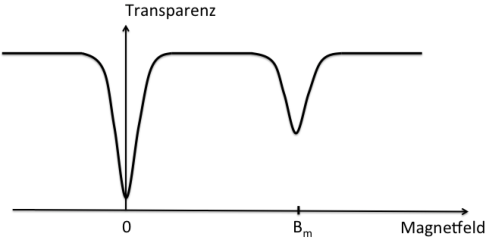
\includegraphics[width=0.6\textwidth]{Abb10.pdf}
	\caption[Transparenz]{Transparenz des Alkali-Gases in einem von außen angelegtem Magnetfeld, um die Resonanzfrequenz zu treffen \cite{\V}}
	\label{fig:transparenz}
\end{figure}
Die Resonanzstelle kann gut durch die Transparenz des Gases gefunden werden (siehe Abb. \ref{fig:transparenz}). Das Gas wird permanent mit rechtszirkular polarisiertem Licht bestrahlt. Ab dem Moment wenn die Besetzungsinversion einsetzt, ist das Gas transparent. Wenn nun die induzierte Emission eintritt, ist das Grundniveau wieder besetzt und das einfallende Licht hebt die Elektronen auf einen höheren Zustand. Solange das Grundniveau besetzt ist, ist das Gas nicht vollständig transparent. \\
Der Versuchsaufbau, um die Resonanzen zu finden ist in Abb. \ref{fig:aufbau} dargestellt. Die Spektrallampe liefert das Licht, um die Elektronen anzuregen. Das Licht wird in einem Polarisator rechtszirkular polarisiert und mit einer Sammellinse auf das Alkali-Gas aus Rubidium-85 und Rubidium-87 Isotopen fokussiert. Das erhitzte Alkali-Gas befindet sich im thermodynamischen Gleichgewicht. Der Kolben ist von drei Holmholtz-Spulen umgeben und einer Spule, die die Hochfrequenz generiert. Die Frequenz wird immer auf einen festen Wert zwischen \si{100}{\kilo\hertz} und \si{1}{\mega\hertz} eingestellt und das Magnetfeld fährt einen Bereich kontinuierlich durch (Modulationsfeldspule). Auf der anderen Seite des Kolbens ist eine Diode, die an ein Oszilloskop angeschlossen ist. 
\begin{figure}[H]
	\centering
	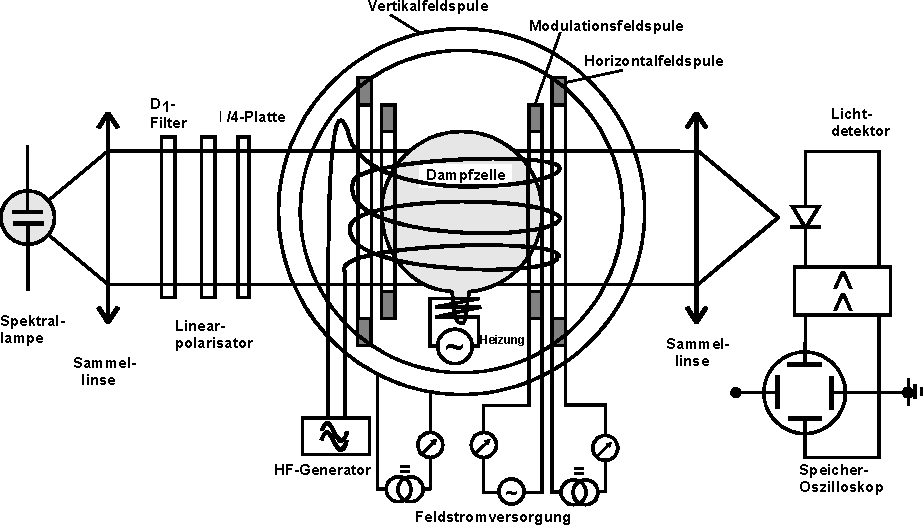
\includegraphics[width=\textwidth]{Abb13.pdf}
	\caption{Versuchsaufbau \cite{\V}}
	\label{fig:aufbau}
\end{figure}


\subsection{Durchführung}
Insgesamt wird eine Messreihe und ein Bild aufgenommen. In der Messreihe werden die Frequenzen und Magnetfelder an der Resonanzstelle der beiden verschiedenen Isotope aufgenommen. Das Bild zeigt den Spannungsverlauf am Oszilloskop, der die typische Transparenzkurve darstellt. Die einzelnen Schritte der Vorbereitung und der Messung sind folgende:
\begin{enumerate}
	\item Der Strahlengang wird durch die Sammellinsen so aufgebaut, dass das die Diode eine maximale Spannung ausgibt. 
	\item Das Magnetfeld wird berücksichtigt. Die horizontale Komponente wird durch Drehen des gesamten Aufbaus verändert und die vertikale durch die vertikale Helmholtz-Spule. Beides wird so eingestellt, dass die ansteigende Flanke der Transparenz-Kurve möglichst steil ist. 
	\item Für den Frequenzbereich \si{100}{\kilo\hertz} bis \si{1}{\mega\hertz} wird in Abständen von \si{100}{\kilo\hertz} die Resonanzstelle beider Isotope gesucht. Dafür verwendet man die Modulationsfeldspule. Reicht der Bereich der Modulationsfeldspule nicht aus, wird zusätzlich ein Magnetfeld durch die horizontale Helmhotz-Spule angelegt.
	\item Ein Bild eines typischen Signalverlaufs soll aufgenommen werden.
\end{enumerate}


